% 图表插入清单：共 26 张矢量 PDF。数据图由 figures/gen_fig_*.py 生成；技术路线、
% 四问流程与判据决策共 6 张由 figures/fig_*.html 经 Electron printToPDF 出图。
% 宽度由 _utils/fig_include_size.py --strict 按长宽比与文字密度规整，逻辑框图
% 声明得更窄以抬高折算印刷字号，全部不低于 8pt 下限；数据图保持 0.9\textwidth。
% 需要 [H] 定位，正文导言区须有 \usepackage{float}。
%
% 图注承担「口径与出处」：按 Step 3.45，图内只留必要数值与短锚点，凡结论性、
% 因果性、口径限定的说明一律写在这里，不进绘图区。

% ── 技术路线 ─────────────────────────────────────────────────────────
\begin{figure}[H]
  \centering
  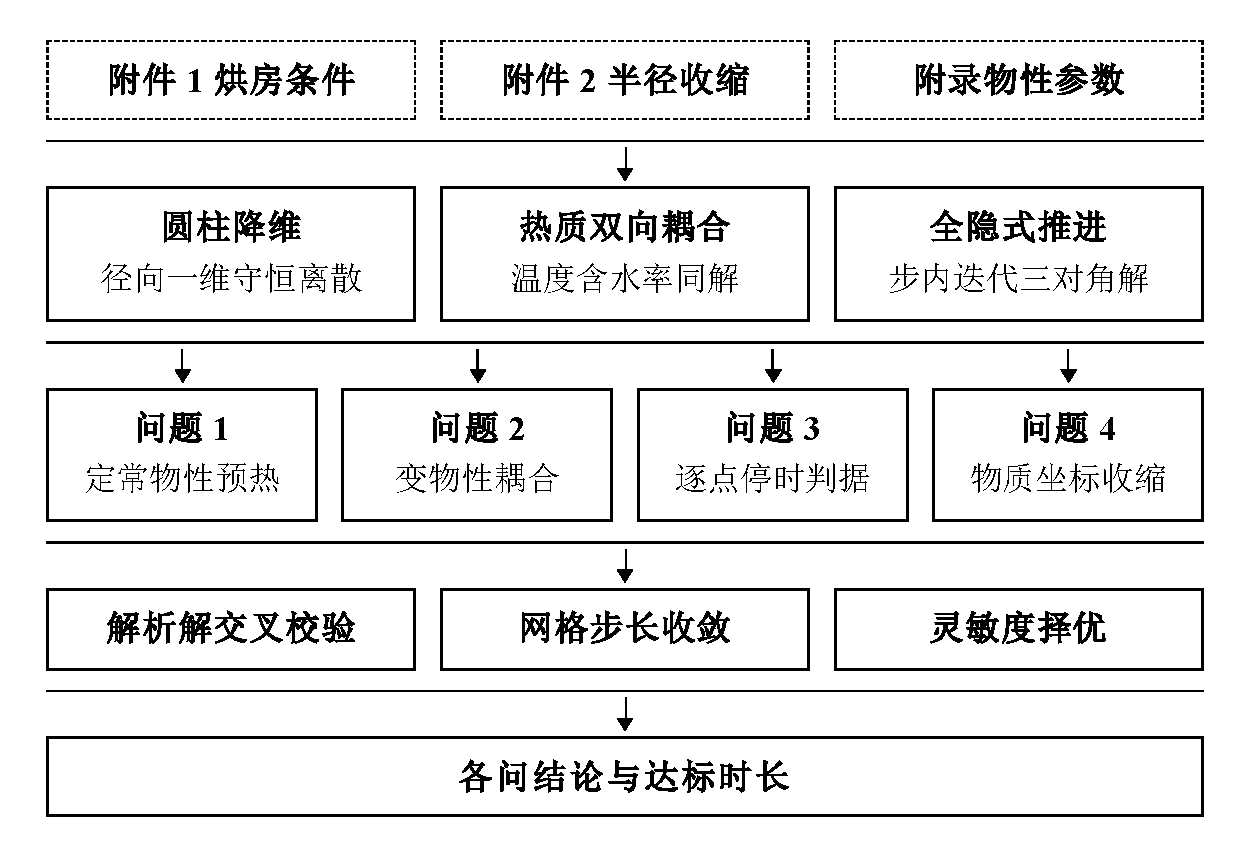
\includegraphics[width=0.8\textwidth,height=0.8\textheight,keepaspectratio]{figures/fig_roadmap.pdf}
  \caption{全文技术路线。自上而下依次为题给数据、四问共用的数学内核、四个问题
  的分支求解、可信性校验与结论交付五层；虚线框表示题给数据，加粗框为四问共用的
  耦合内核，层间横线表示先汇总再分发；四个问题框内第二行即该问在内核之上新增的
  处理，可见四问同源而分支互不重复。}
  \label{fig:roadmap}
\end{figure}

% ── 题面数据 ─────────────────────────────────────────────────────────
\begin{figure}[H]
  \centering
  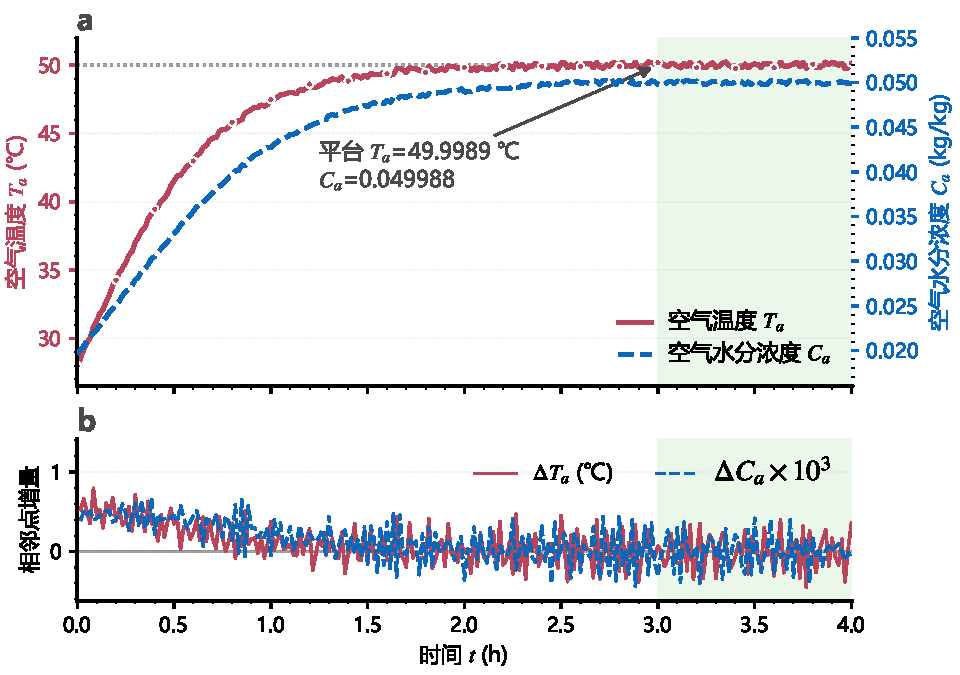
\includegraphics[width=0.9\textwidth,height=0.8\textheight,keepaspectratio]{figures/fig_oven_input.pdf}
  \caption{附件 1 给出的烘房运行条件（241 点实测，未作平滑）。a：空气温度
  $T_a$ 先升温后维持恒定，空气水分浓度 $C_a$ 与之反向变化，两者是表面两个
  Robin 边界的驱动量；b：逐点一阶差分，末段 61 点的增量落在零线附近，据此
  判定序列已进入恒定平台，平台均值用于时间超出实测区间后的延拓。}
  \label{fig:oven-input}
\end{figure}

\begin{figure}[H]
  \centering
  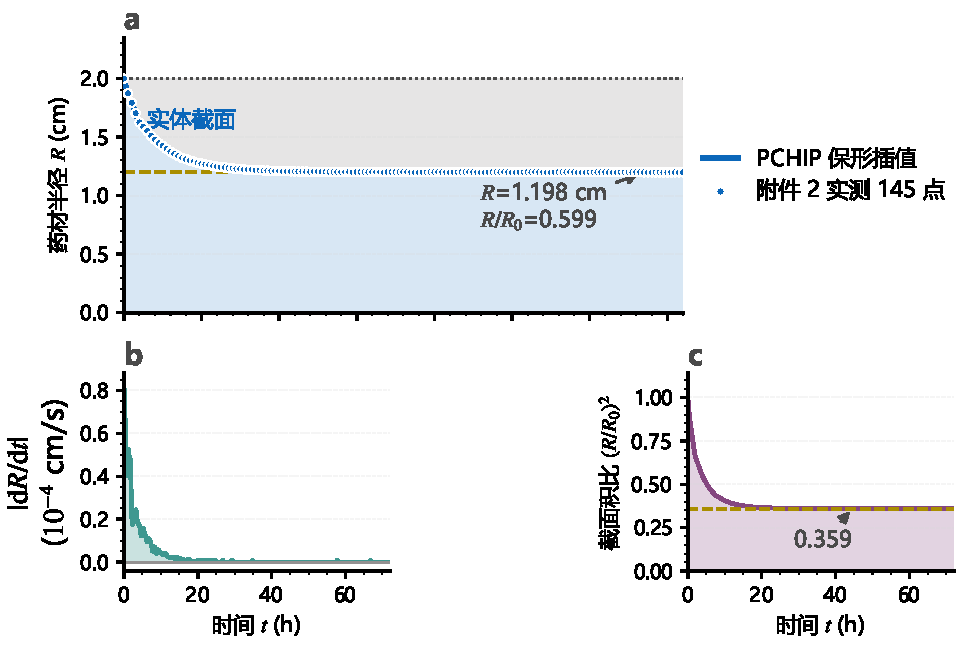
\includegraphics[width=0.9\textwidth,height=0.8\textheight,keepaspectratio]{figures/fig_radius_shrink.pdf}
  \caption{附件 2 实测的药材半径收缩过程。a：散点为 145 点实测值，曲线为
  PCHIP 保形插值（保形以避免插值曲线出现非物理的半径回弹），深色填充为药材
  实体截面，浅色为已收缩掉的区域；b：收缩速率 $|\mathrm{d}R/\mathrm{d}t|$；
  c：截面积比 $(R/R_0)^2$。终值半径与收缩比直接进入问题 4 的物质坐标变换。}
  \label{fig:radius-shrink}
\end{figure}

\begin{figure}[H]
  \centering
  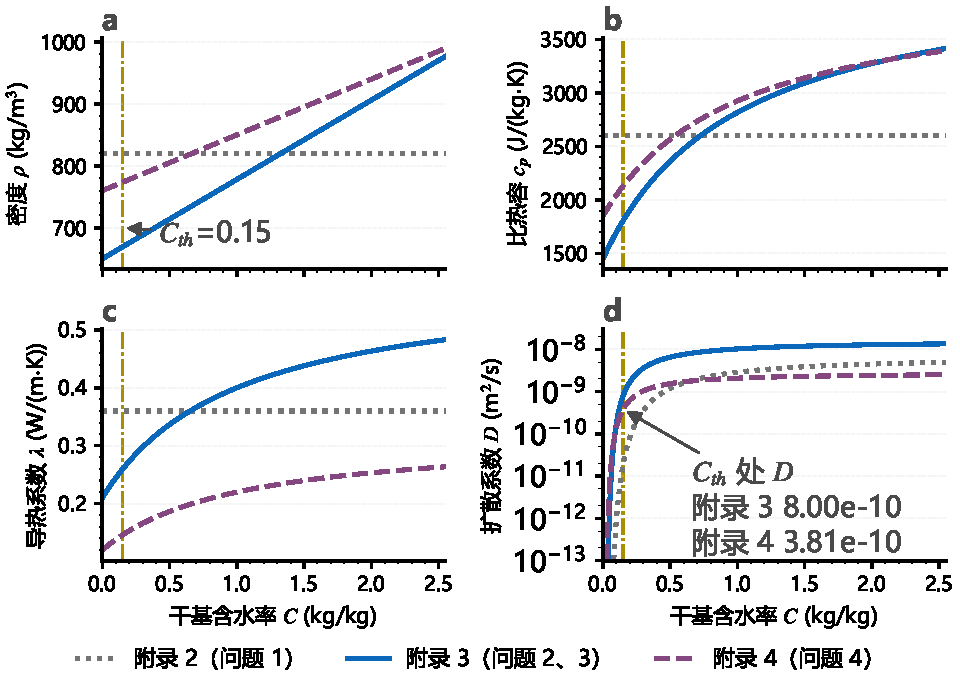
\includegraphics[width=0.9\textwidth,height=0.8\textheight,keepaspectratio]{figures/fig_prop_curves.pdf}
  \caption{附录 2/3/4 三套物性的逐项对照，横轴为干基含水率，点划线标出判据
  阈值 $C_{th}=0.15$ 的位置。a—c：密度、比热容、导热系数；附录 2 为常物性，
  附录 3/4 随含水率变化（比热与导热按湿基 $C/(C{+}1)$ 取值）。d：扩散系数取
  对数纵轴，跨越四个数量级，是三套物性中差异最大的一项，也是问题 4 与问题 3
  停时不同的主要来源。曲线全部由 \texttt{code/utils.Props} 按附录公式现算。}
  \label{fig:prop-curves}
\end{figure}

\begin{figure}[H]
  \centering
  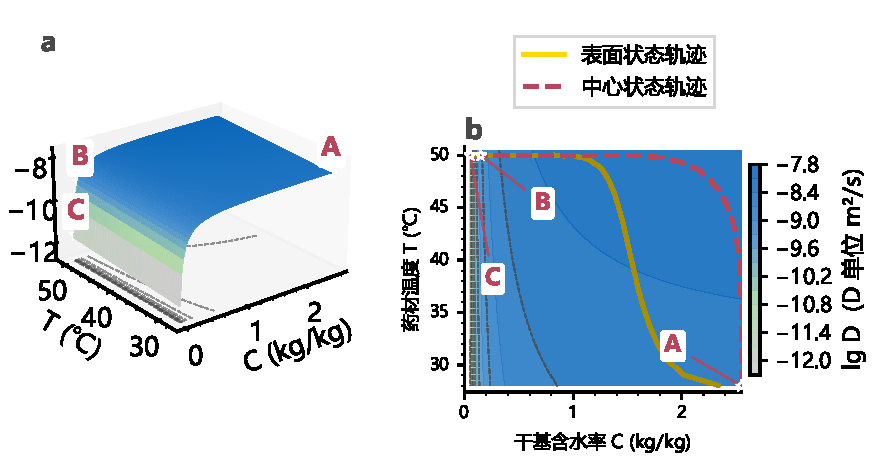
\includegraphics[width=0.9\textwidth,height=0.8\textheight,keepaspectratio]{figures/fig_diff_surface.pdf}
  \caption{附录 3 扩散系数 $D(C,T)$ 的三维曲面与俯视投影。a：$\lg D$ 在
  $(C,T)$ 平面上的曲面，温度经 Arrhenius 因子起主导作用，含水率的修正相对
  次要；A、B、C 三点为问题 3 生产算例实际经过的状态（初始态、判据达标态、
  终态），全称见正文。b：同一函数的等高线俯视图，叠加问题 3 中心与表面状态
  点的实算轨迹，可见两条轨迹在温度维度上先分离后合拢。}
  \label{fig:diff-surface}
\end{figure}

% ── 公共机理 ─────────────────────────────────────────────────────────
\begin{figure}[H]
  \centering
  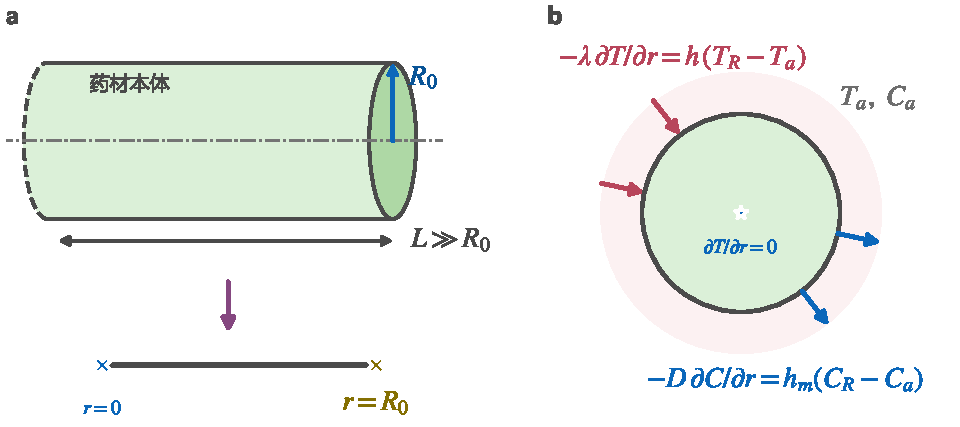
\includegraphics[width=0.9\textwidth,height=0.8\textheight,keepaspectratio]{figures/fig_mech_geometry.pdf}
  \caption{几何降维与边界条件。长径比足够大时轴向与周向梯度可略，三维圆柱
  问题降为一维径向问题；表面同时承担对流换热与对流传质两个 Robin 条件，
  轴线处由对称性给出零通量。}
  \label{fig:mech-geometry}
\end{figure}

\begin{figure}[H]
  \centering
  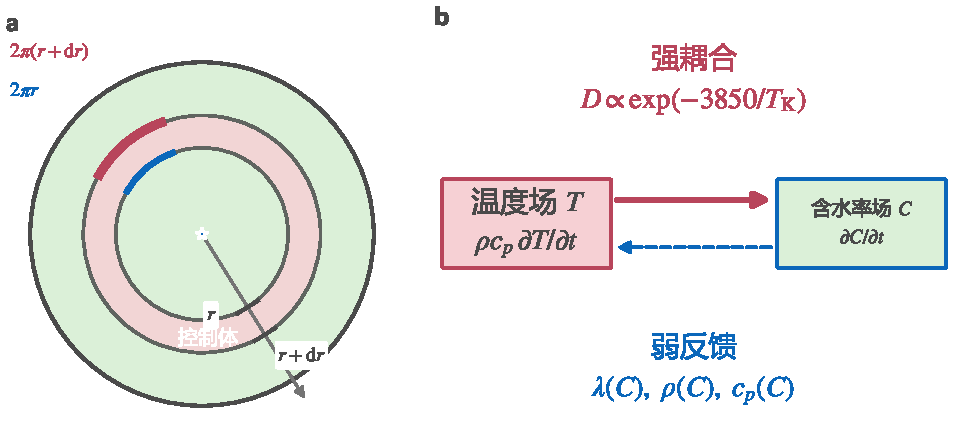
\includegraphics[width=0.9\textwidth,height=0.8\textheight,keepaspectratio]{figures/fig_mech_coupling.pdf}
  \caption{守恒律的面积加权与双向耦合。环形控制体内外两个柱面的通过面积不
  相等，这是圆柱几何区别于平板的根源，整理后在方程中留下面积加权项；温度对
  扩散系数是强耦合，含水率对热物性只是弱反馈。}
  \label{fig:mech-coupling}
\end{figure}

\begin{figure}[H]
  \centering
  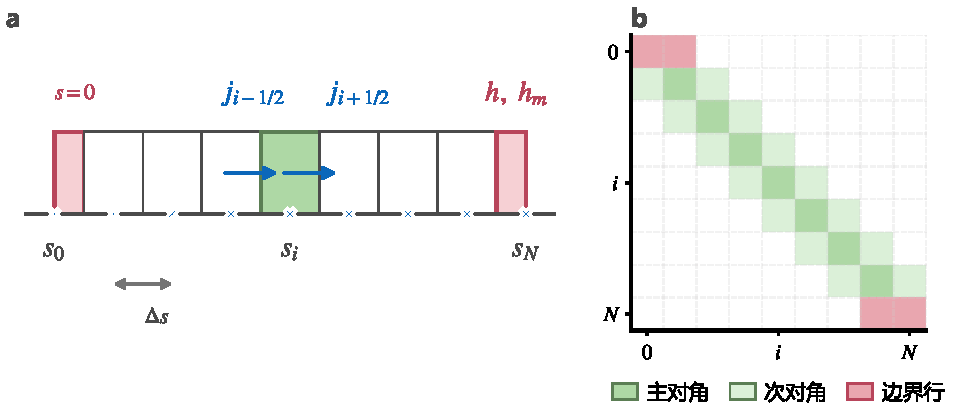
\includegraphics[width=0.9\textwidth,height=0.8\textheight,keepaspectratio]{figures/fig_mech_fvm.pdf}
  \caption{顶点式有限体积网格与代数结构。节点落在输出要求的位置上，两端为
  半控制体；内侧界面的面积因子为零使轴线零通量精确满足，不需虚节点，由此得
  到的系数矩阵严格三对角。图中网格数仅为作图清晰，不代表实算网格。}
  \label{fig:mech-fvm}
\end{figure}

\begin{figure}[H]
  \centering
  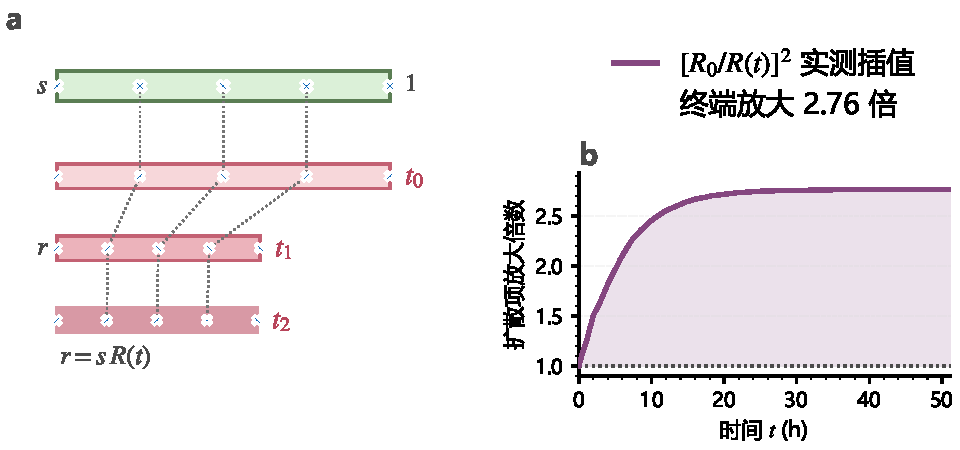
\includegraphics[width=0.9\textwidth,height=0.8\textheight,keepaspectratio]{figures/fig_mech_moving.pdf}
  \caption{物质坐标映射与收缩放大。a：固定域上的节点随物质一起向轴线移动，
  表观对流项与坐标变换项精确相消，方程中不出现半径变化率；点线为同一物质点
  在三个时刻的轨迹。b：收缩以半径平方的倒数进入扩散项，放大倍数由附件 2
  实测半径算出，这是收缩加速干燥的数学来源。}
  \label{fig:mech-moving}
\end{figure}

% ── 问题 1：预热平衡 ─────────────────────────────────────────────────
\begin{figure}[H]
  \centering
  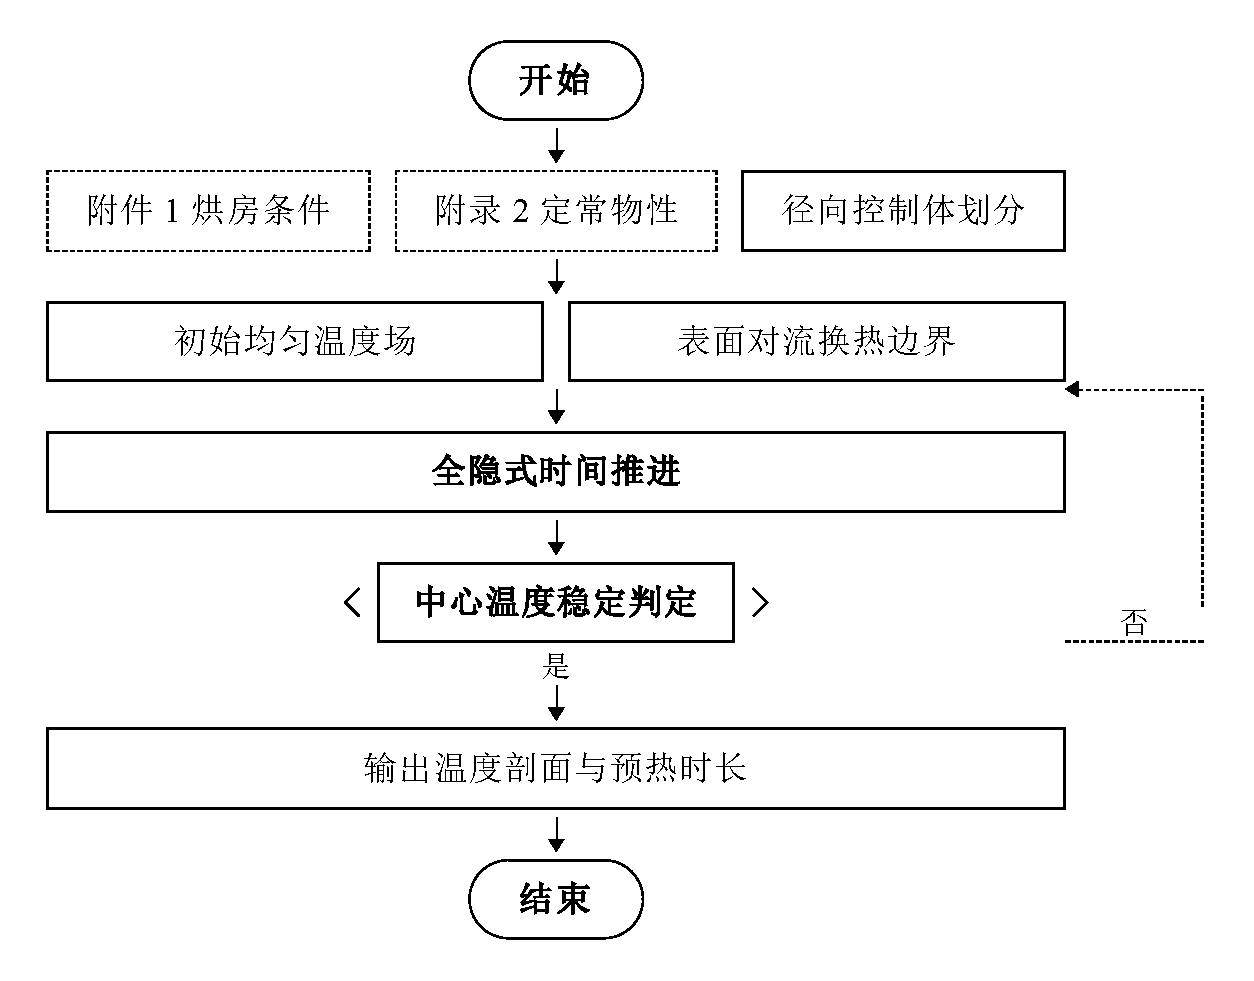
\includegraphics[width=0.8\textwidth,height=0.8\textheight,keepaspectratio]{figures/fig_flow_q1.pdf}
  \caption{问题 1 的求解流程。自上而下为数据与网格准备、初始与边界设定、全隐式
  时间推进三段，虚线框表示题给数据，加粗框为主控步骤；右侧虚线回路表示中心温度
  未达稳定时返回继续推进，达稳定后输出温度剖面与预热时长。}
  \label{fig:flow-q1}
\end{figure}

\begin{figure}[H]
  \centering
  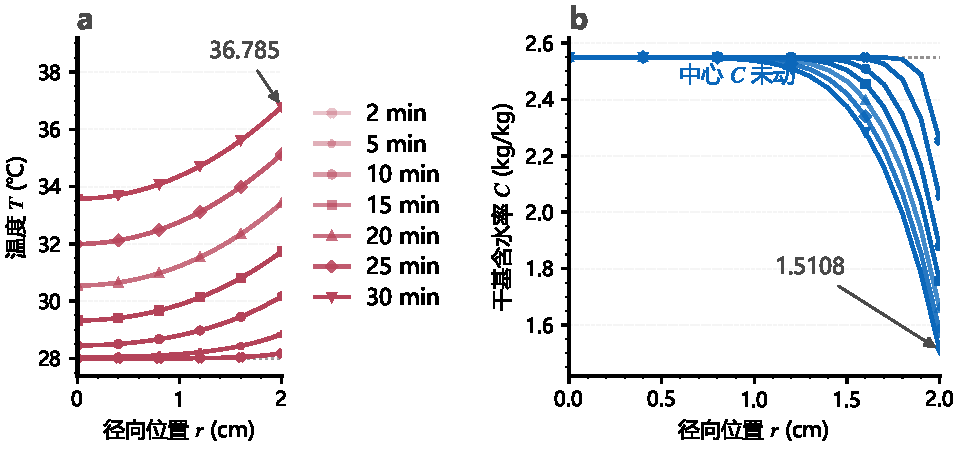
\includegraphics[width=0.9\textwidth,height=0.8\textheight,keepaspectratio]{figures/fig_q1_profiles.pdf}
  \caption{预热阶段的径向剖面族，7 个输出时刻用同族深浅渐变区分，径向取 21
  个位置（0.1\,cm 间隔）。a：温度剖面自初始均匀态由外向内抬升，表面始终领先
  于中心，中心的追赶速度决定预热时长；b：同期含水率剖面只有表层下降，中心在
  30\,min 内几乎未动——这一快慢分离说明预热段可只看温度判平衡。}
  \label{fig:q1-profiles}
\end{figure}

\begin{figure}[H]
  \centering
  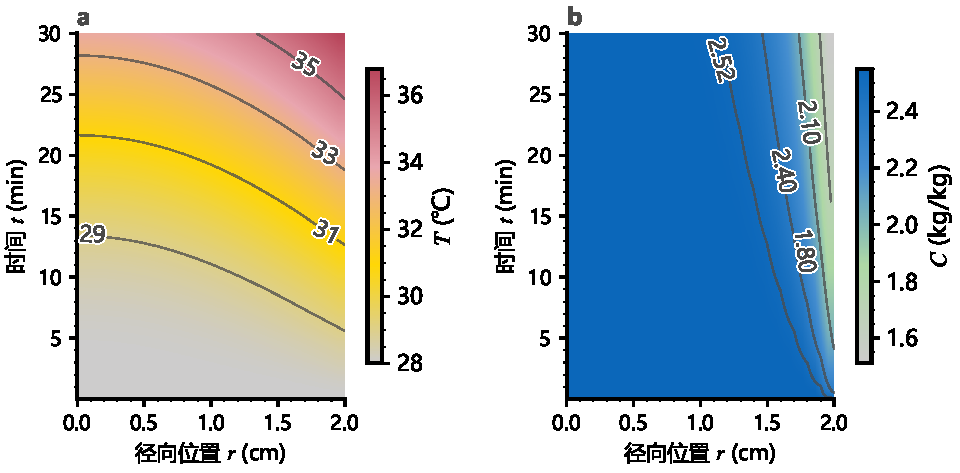
\includegraphics[width=0.9\textwidth,height=0.8\textheight,keepaspectratio]{figures/fig_q1_hovmoller.pdf}
  \caption{预热阶段温度场与水分场的时间—半径分布（$200\times21$ 输出网格）。
  a：温度等值线自表面向轴线推进，可读出热波到达轴线的时刻与其后的整体抬升；
  b：同期水分场，等值线几乎平行于时间轴，说明 30\,min 内水分尚未形成贯穿性
  梯度。两幅同尺度并置，用于对比热扩散与质扩散的时间尺度差异。}
  \label{fig:q1-hovmoller}
\end{figure}

\begin{figure}[H]
  \centering
  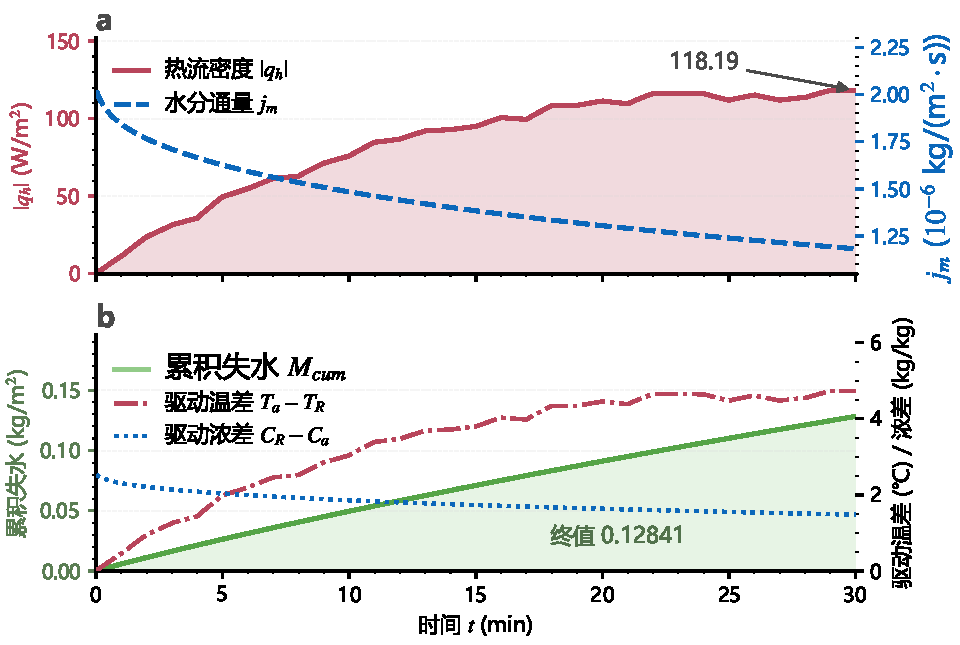
\includegraphics[width=0.9\textwidth,height=0.8\textheight,keepaspectratio]{figures/fig_q1_flux.pdf}
  \caption{预热阶段表面通量与累积失水（1\,s 输出，1800 点）。a：热流密度
  $|q_h|$ 随表面与空气温差缩小而单调衰减，水分通量 $j_m$ 反而上升，因表面
  升温抬高了平衡含湿的差值；b：累积失水量与两个驱动力（温差、浓差）的同步
  演化，驱动温差衰减而驱动浓差近似持平，故失水近似线性累积。}
  \label{fig:q1-flux}
\end{figure}

% ── 问题 2：全过程 ───────────────────────────────────────────────────
\begin{figure}[H]
  \centering
  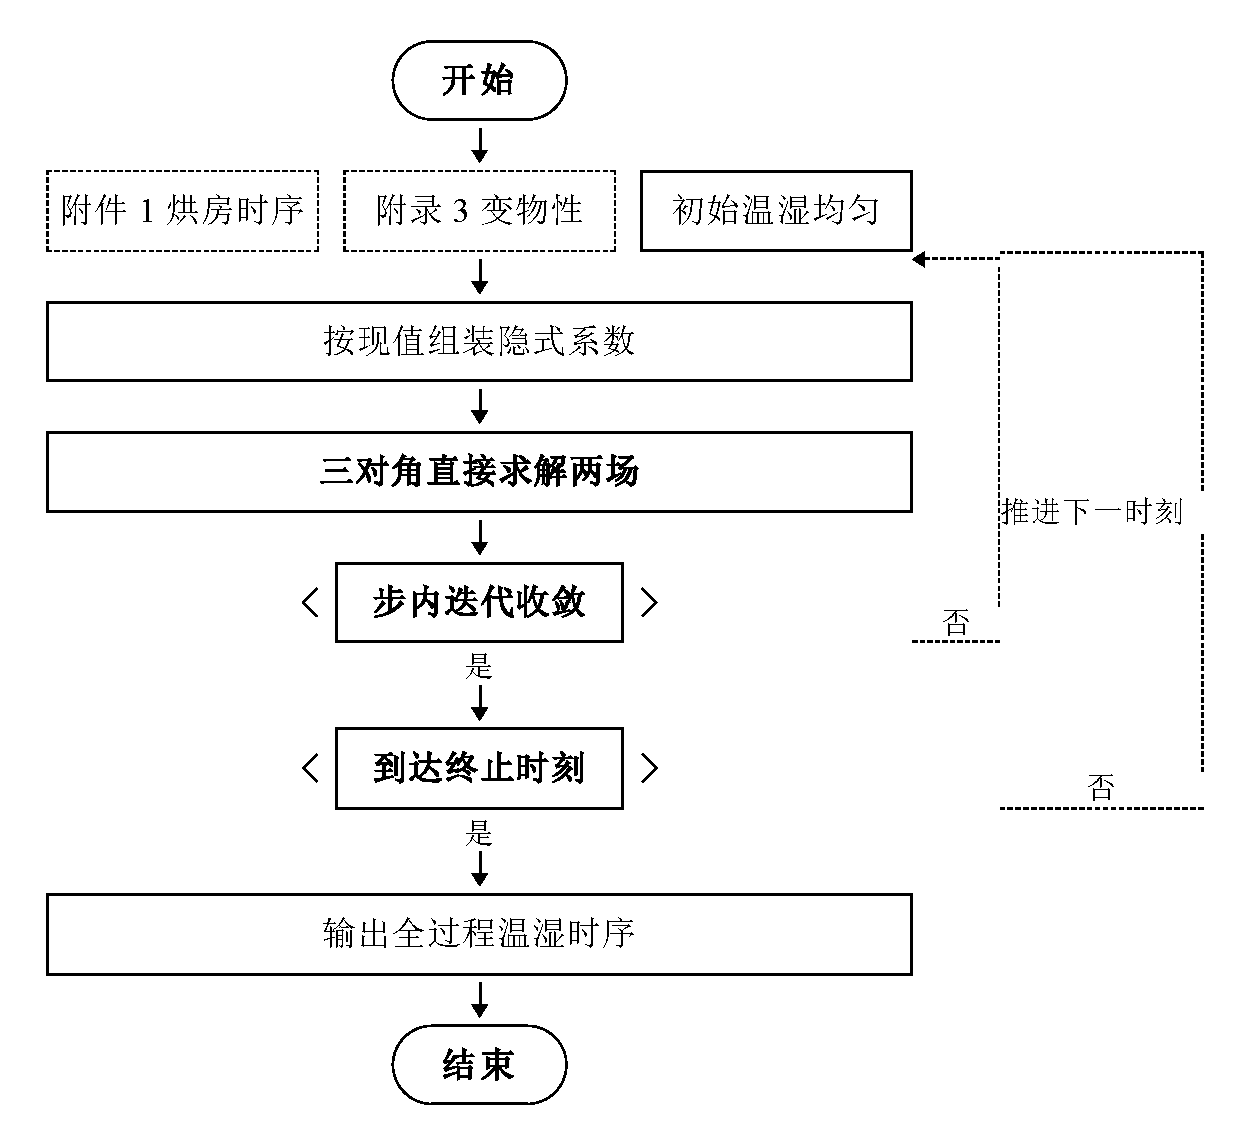
\includegraphics[width=0.86\textwidth,height=0.8\textheight,keepaspectratio]{figures/fig_flow_q2.pdf}
  \caption{问题 2 全过程求解的双重迭代结构。主链是一次时间步内的动作；内侧回路
  为步内 Picard 非线性迭代，外侧回路为步间时间推进，两条回路都返回到系数组装，
  区别在于外侧回路先推进到下一时刻。虚线框表示题给数据。}
  \label{fig:flow-q2}
\end{figure}

\begin{figure}[H]
  \centering
  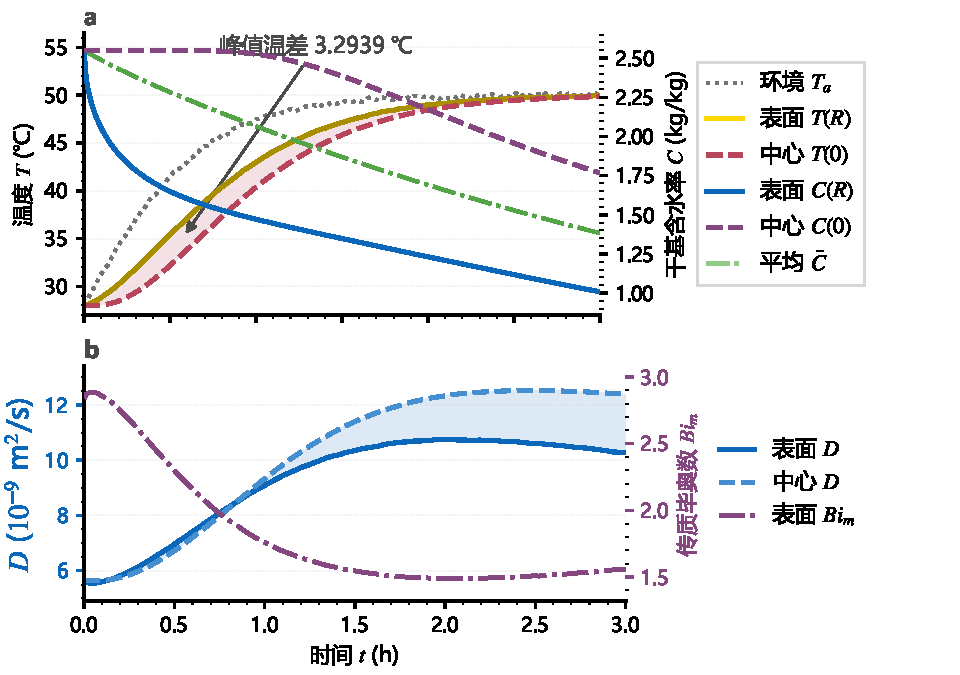
\includegraphics[width=0.9\textwidth,height=0.8\textheight,keepaspectratio]{figures/fig_q2_dual.pdf}
  \caption{问题 2 前三小时的双轴演化与变物性响应。a：中心与表面温度追随空气
  温度上升，阴影为中心—表面温差带，同期三条含水率曲线同步下降；温度很快进入
  准稳态，含水率的下降贯穿整个过程，两者时间尺度相差一个量级以上。b：表面与
  中心扩散系数、表面传质毕奥数随含水率下降的实时变化——$D$ 在三小时内变化近
  一倍，故变物性不能用常数近似替代。}
  \label{fig:q2-dual}
\end{figure}

\begin{figure}[H]
  \centering
  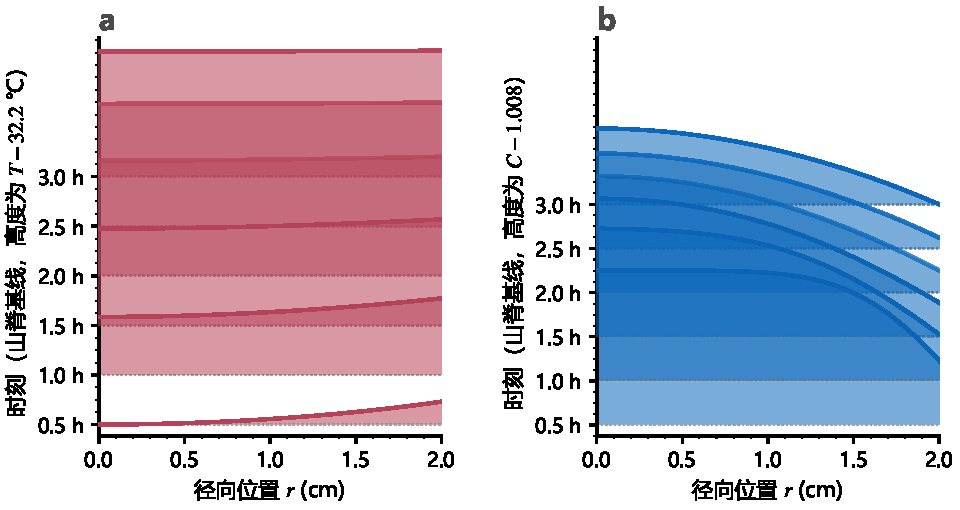
\includegraphics[width=0.9\textwidth,height=0.8\textheight,keepaspectratio]{figures/fig_q2_ridgeline.pdf}
  \caption{问题 2 径向剖面的山脊图，6 个整时刻沿纵深方向排开（0.5\,h 间隔，
  21 个径向位置），纵向偏移即时间，每条山脊的高度是该时刻剖面相对全场最小值
  的抬升量。a：温度；b：含水率。干燥自表面向内推进，表面与轴线的落差先增大
  后随整体变干而趋缓，最湿位置始终在轴线附近——这是问题 3 采用逐点最大判据的
  直接依据。山脊排布用于避免六条剖面互相压线。}
  \label{fig:q2-ridgeline}
\end{figure}

% ── 问题 3：停时判定 ─────────────────────────────────────────────────
\begin{figure}[H]
  \centering
  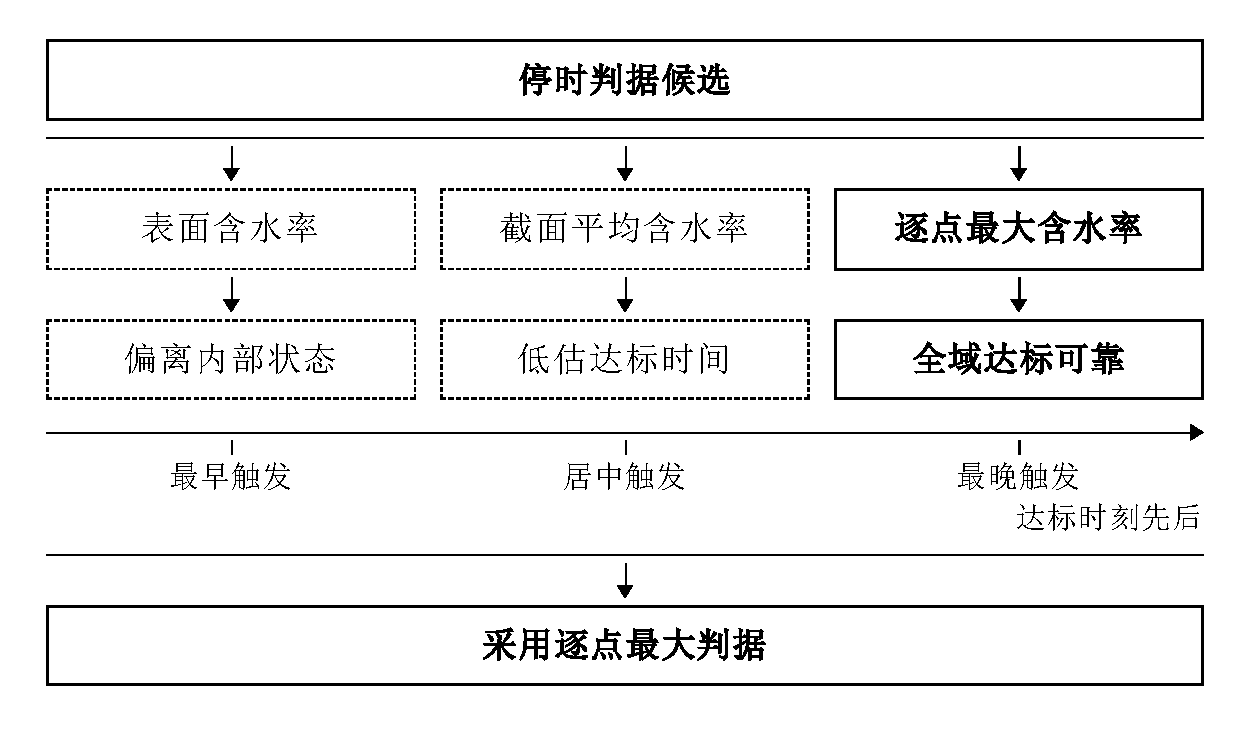
\includegraphics[width=0.9\textwidth,height=0.8\textheight,keepaspectratio]{figures/fig_criterion_logic.pdf}
  \caption{停时判据的三候选决策。表面判据偏离内部状态，截面平均判据会低估达
  标时间，逐点最大判据能保证全域达标，故取后者；加粗框为采纳路径，虚线框为对照
  路径。底部时间轴只表示三种判据触发的先后次序，不含数值。}
  \label{fig:criterion-logic}
\end{figure}

\begin{figure}[H]
  \centering
  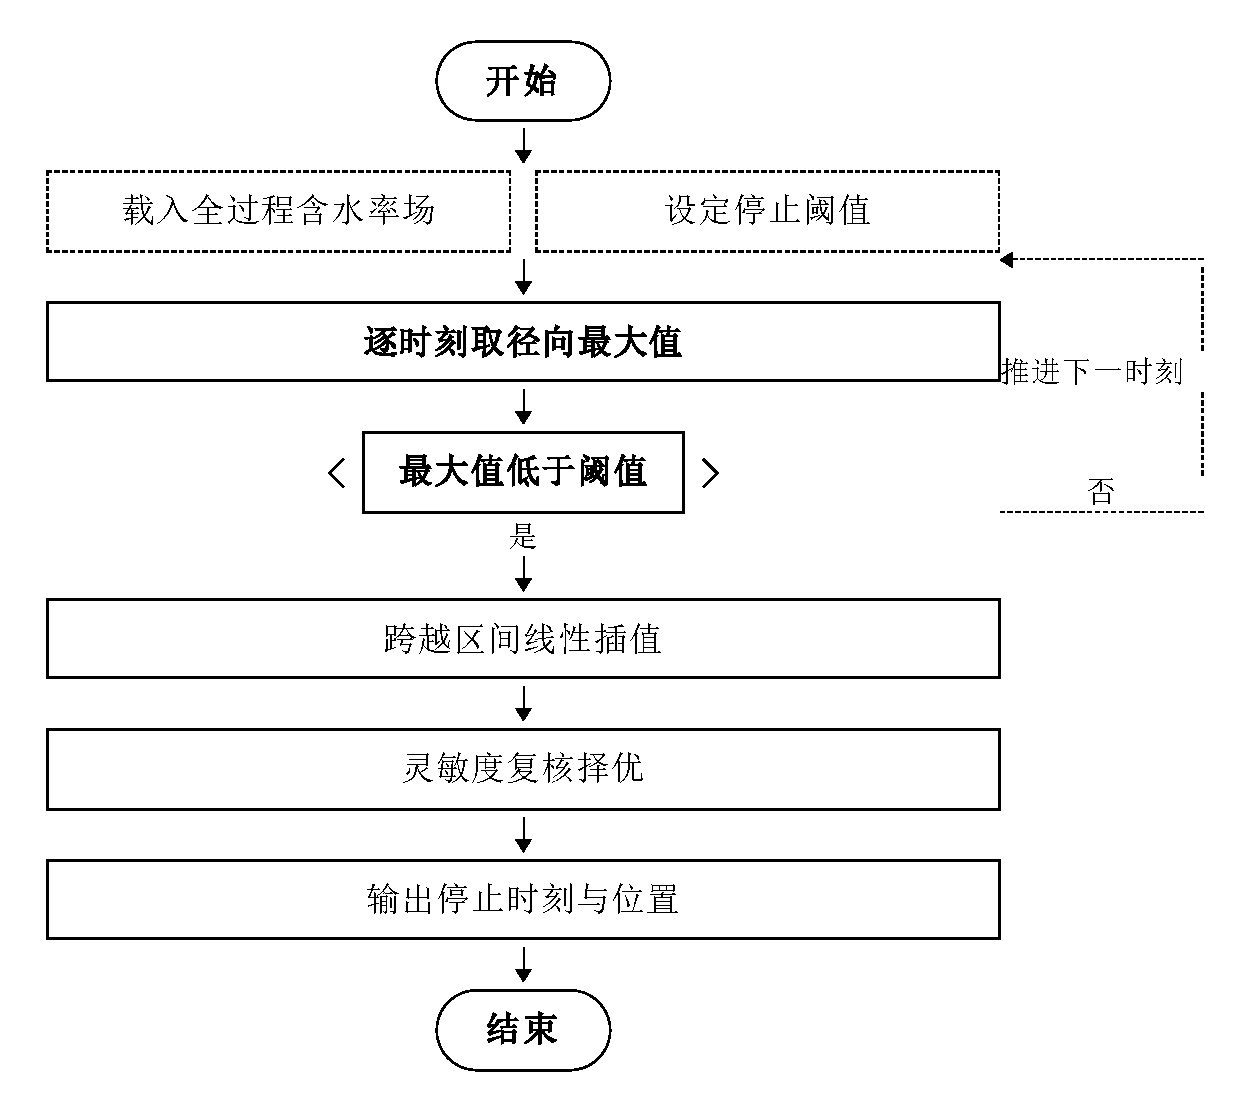
\includegraphics[width=0.86\textwidth,height=0.8\textheight,keepaspectratio]{figures/fig_flow_q3.pdf}
  \caption{问题 3 停止时刻的判定流程。逐时刻取径向最大含水率与阈值比较，未达
  阈值则由右侧回路推进到下一时刻，已达阈值则在跨越区间内线性插值定位停时，再经
  灵敏度复核后输出。虚线框表示题给数据与外部设定的阈值口径。}
  \label{fig:flow-q3}
\end{figure}

\begin{figure}[H]
  \centering
  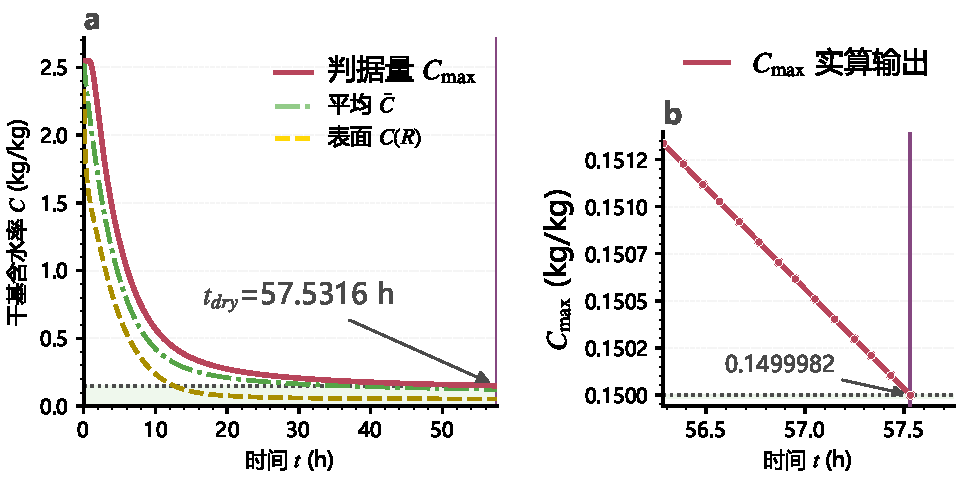
\includegraphics[width=0.9\textwidth,height=0.8\textheight,keepaspectratio]{figures/fig_q3_criterion.pdf}
  \caption{问题 3 停时判据的实算依据。a：判据量 $\max_r C$、表面含水率与截面
  平均含水率三条曲线的全程下降，水平点线为阈值 0.15，绿色底带为达标区；三条
  曲线的先后次序印证了平均判据偏早、表面判据更偏早。b：停时前 1.25\,h 的邻域
  放大（1\,min 分辨率的实算输出点），显示判据被单调穿越且只穿越一次，故插值
  定位的停时唯一。轴对称条件下最湿位置恒在轴线，$\max_r C$ 即中心值。}
  \label{fig:q3-criterion}
\end{figure}

\begin{figure}[H]
  \centering
  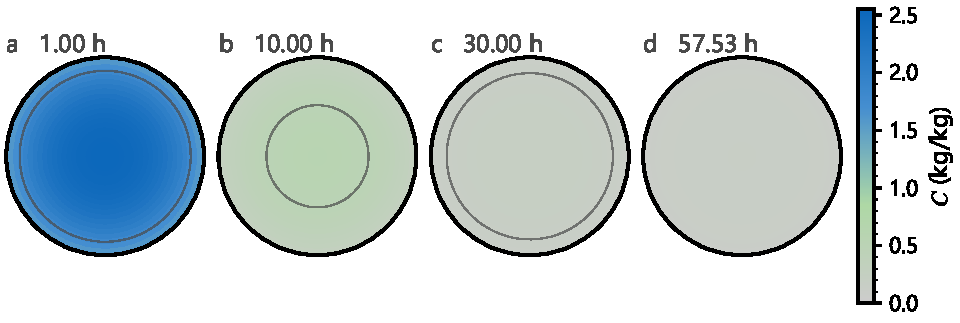
\includegraphics[width=0.9\textwidth,height=0.8\textheight,keepaspectratio]{figures/fig_q3_frames.pdf}
  \caption{问题 3 圆截面水分场的四帧俯视快照（1、10、30\,h 与停时），把一维
  径向解按轴对称铺成圆盘。四帧共用同一色标以便跨帧比较，细等值线为 0.15、
  0.5、1.0、1.8 四级。干燥前沿由外向内推进，末帧整盘进入达标色域，直观说明
  全域达标是在最湿的轴线越过阈值那一刻实现的。}
  \label{fig:q3-frames}
\end{figure}

% ── 问题 4：收缩域 ───────────────────────────────────────────────────
\begin{figure}[H]
  \centering
  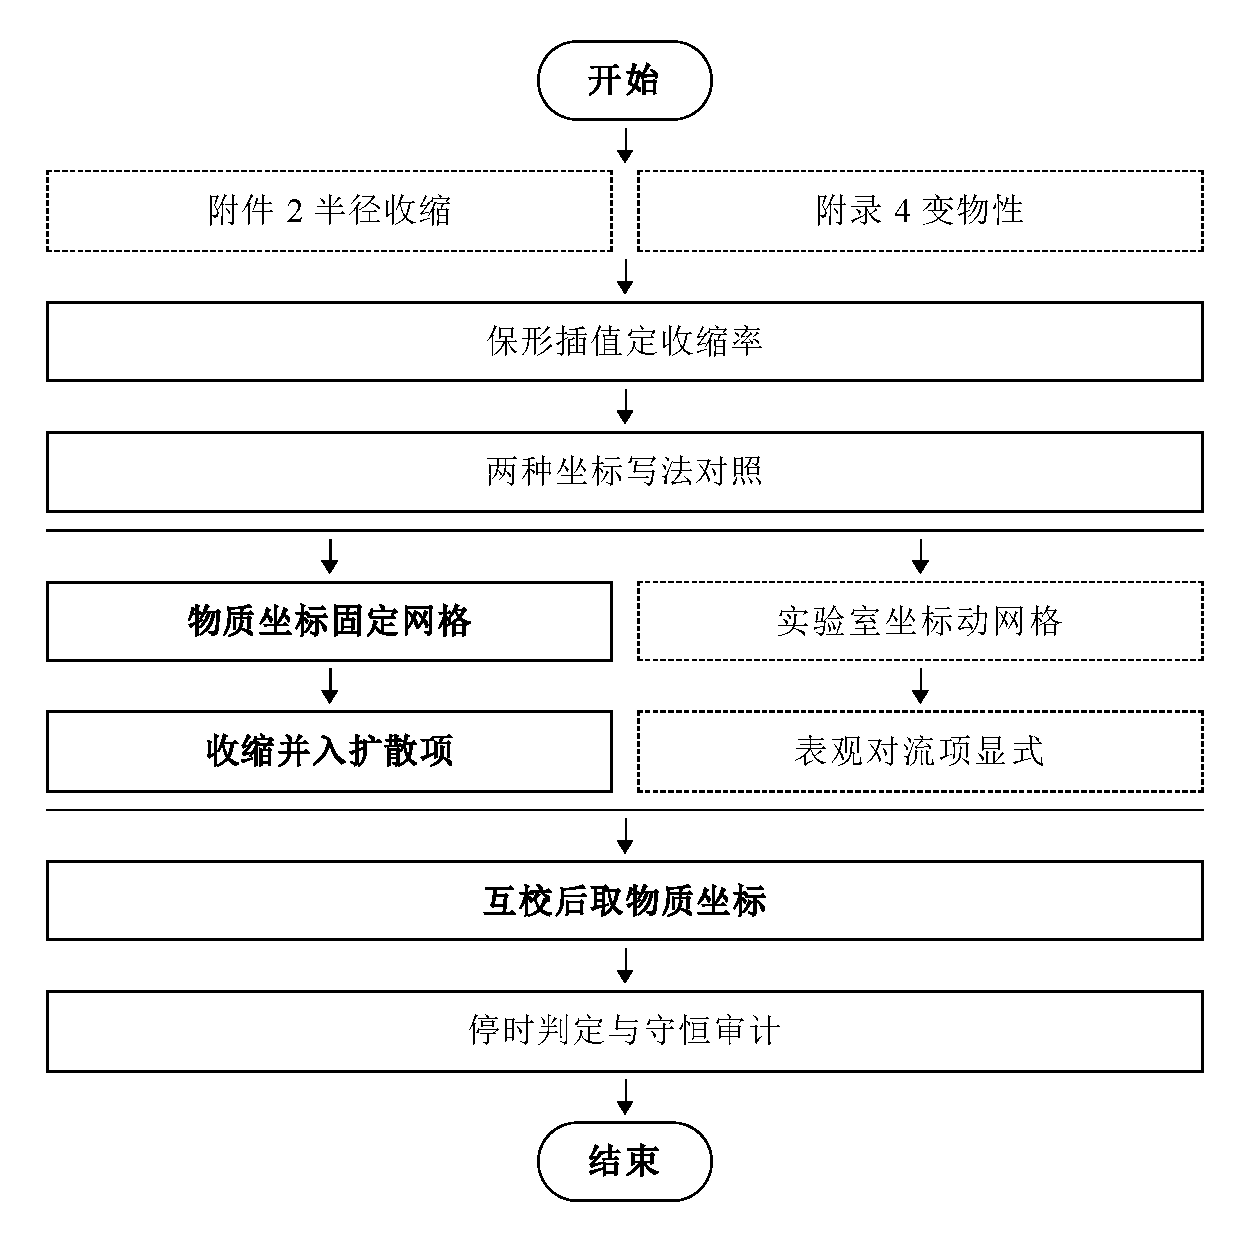
\includegraphics[width=0.8\textwidth,height=0.8\textheight,keepaspectratio]{figures/fig_flow_q4.pdf}
  \caption{问题 4 收缩域的两条坐标路线。共同输入后分为物质坐标固定网格与实
  验室坐标动网格两支，收缩效应分别并入扩散项与显式表观对流项；加粗框为采纳的
  物质坐标支，虚线框为实验室坐标对照支，两支互校后取前者为主模型，再做停时判定
  与干物质守恒审计。}
  \label{fig:flow-q4}
\end{figure}

\begin{figure}[H]
  \centering
  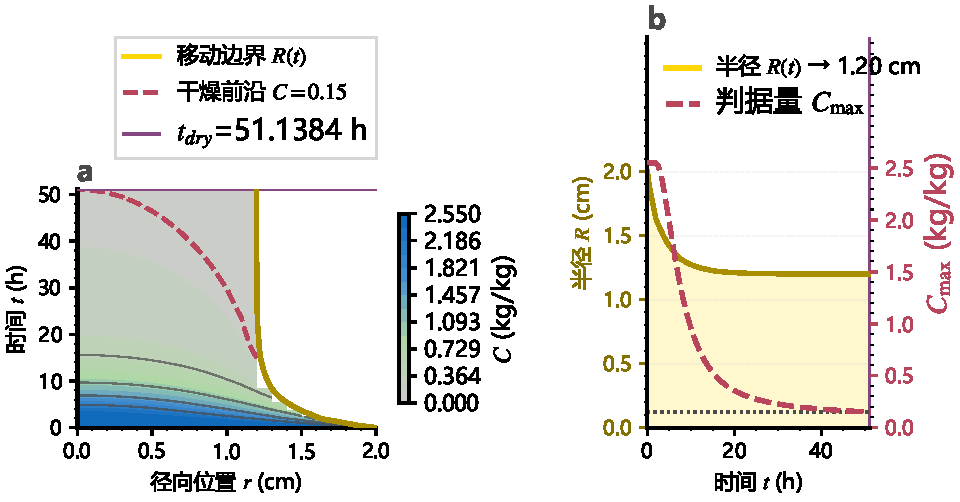
\includegraphics[width=0.9\textwidth,height=0.8\textheight,keepaspectratio]{figures/fig_q4_contour.pdf}
  \caption{问题 4 收缩域内的水分场。a：$(r,t)$ 平面上的含水率等高线，实心区为
  药材本体，移动边界 $R(t)$ 右侧留白即已收缩掉的区域（不填零值以免与"很干"
  混淆）；粗虚线为干燥前沿 $C=0.15$，它与 $R(t)$ 的交汇决定停时。b：半径
  $R(t)$ 与判据量 $C_{\max}$ 的同步演化，竖线为停时；判据量在半径已趋平后
  才穿越阈值，说明停时由水分扩散而非几何收缩直接决定。}
  \label{fig:q4-contour}
\end{figure}

\begin{figure}[H]
  \centering
  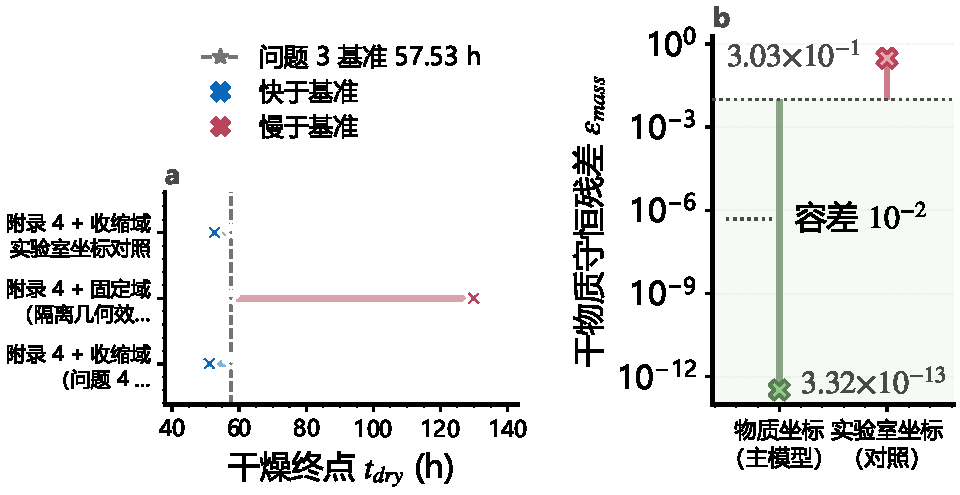
\includegraphics[width=0.9\textwidth,height=0.8\textheight,keepaspectratio]{figures/fig_q34_compare.pdf}
  \caption{问题 3 与问题 4 的效应分解与坐标系审计。a：哑铃图，每行一个分支，
  左端固定为问题 3 的基准停时，右端为该分支实算值，连线长度即该处理的净效应；
  可见单换附录 4 物性（固定域）使干燥显著变慢，再叠加半径收缩才把停时拉回并
  超过基准，两个效应方向相反。b：两种坐标写法的干物质守恒残差，以 $10^{-2}$
  容差线为基线的杆状图（对数纵轴上柱长会随人为地板而变，故不用柱状）；物质
  坐标残差处于机器精度，实验室坐标达 30\%，远超容差，故后者只作对照分支。}
  \label{fig:q34-compare}
\end{figure}

% ── 可信性与择优 ─────────────────────────────────────────────────────
\begin{figure}[H]
  \centering
  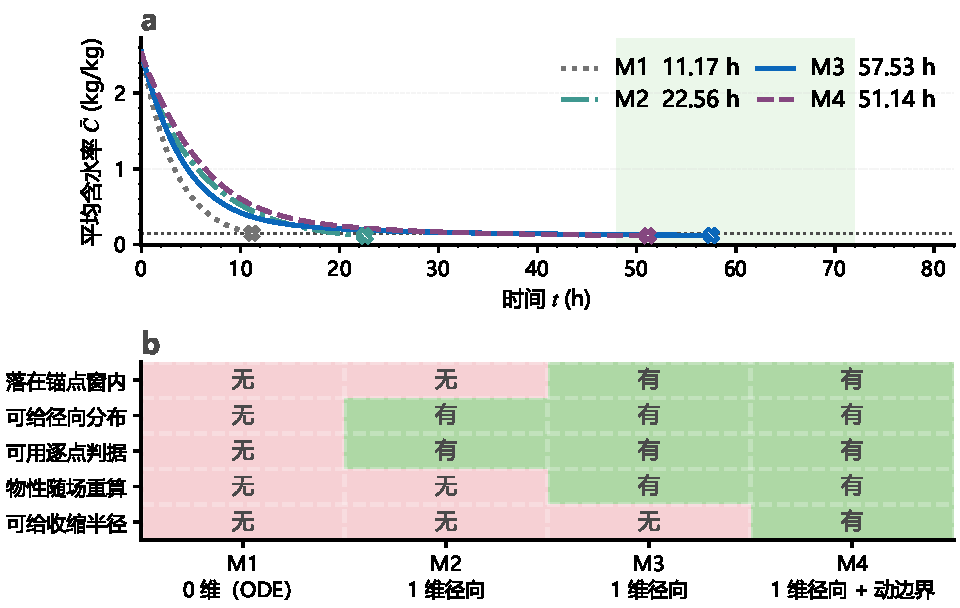
\includegraphics[width=0.9\textwidth,height=0.8\textheight,keepaspectratio]{figures/fig_model_compare.pdf}
  \caption{四个候选模型的横向对比。a：M1—M4 的平均含水率轨迹与各自判据下的
  停时（圆点），灰带为题面所给 2—3 d 外部参考窗口换算的时间区间，只有 M3、
  M4 的停时落在窗内。b：能力矩阵，逐格标记该模型是否具备对应能力；其中"落在
  锚点窗内"一行即指 a 图灰带。逐级叠加常物性、变物性、变物性加收缩三档，可
  分离出各档对停时的贡献，并说明为何取 M4 为主模型。}
  \label{fig:model-compare}
\end{figure}

\begin{figure}[H]
  \centering
  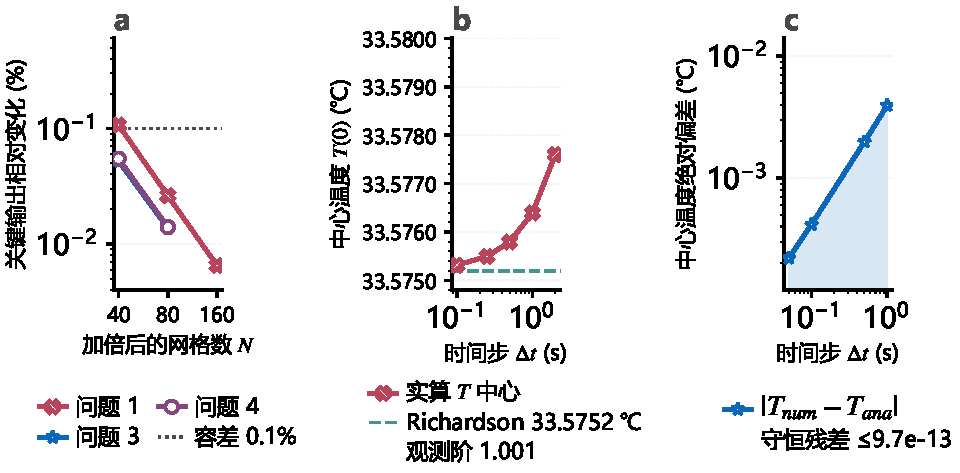
\includegraphics[width=0.9\textwidth,height=0.8\textheight,keepaspectratio]{figures/fig_verification.pdf}
  \caption{数值可信性三联校验。a：三个问题的关键输出在网格加倍下的相对变化，
  全部落在 0.1\% 容差线以下；b：固定网格下中心温度随时间步收敛，观测阶约为 1，
  与后向 Euler 的理论一阶一致，虚线为 Richardson 外推极限；c：常物性算例与十项
  Bessel 级数解析解的中心温度绝对偏差随时间步单调下降。三项合起来说明所报结果
  不依赖离散参数的具体取法。}
  \label{fig:verification}
\end{figure}

\begin{figure}[H]
  \centering
  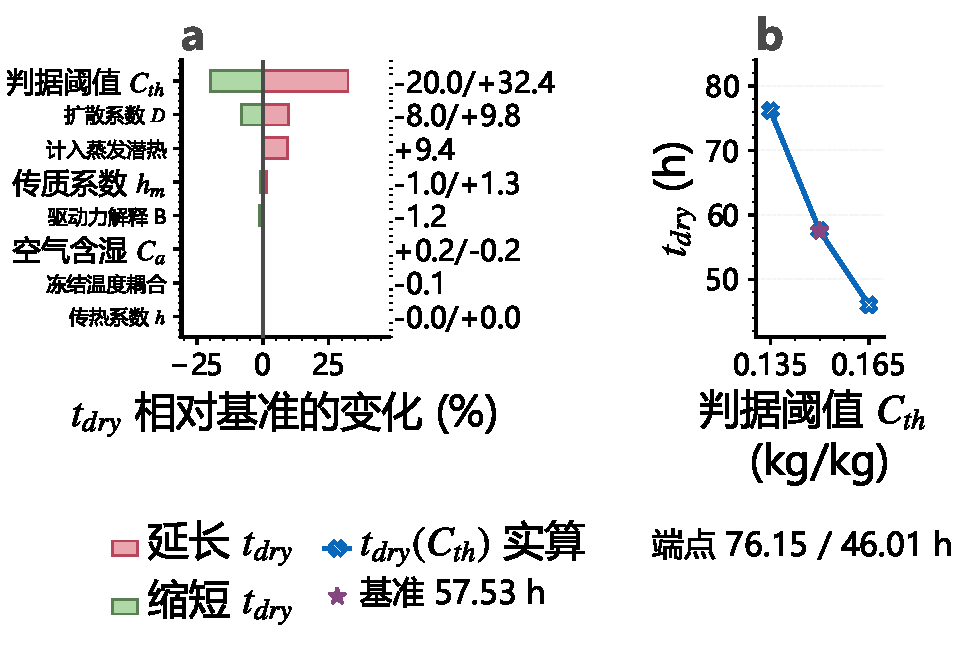
\includegraphics[width=0.9\textwidth,height=0.8\textheight,keepaspectratio]{figures/fig_sensitivity.pdf}
  \caption{问题 3 的灵敏度与鲁棒性。a：龙卷风图，13 个 $\pm10\%$ 扰动算例按
  物理量合并为 8 行并按效应绝对值排序，右侧为延长、左侧为缩短，右侧刻度给出
  两侧的相对变化百分数；扩散系数与判据阈值的效应量级明显领先，传热系数则几乎
  无影响，这与预热远快于干燥的时间尺度分离一致。b：判据阈值的单侧扰动效应明显
  不对称，下调阈值造成的延长幅度大于上调阈值造成的缩短幅度，故阈值口径需在
  正文中明确声明。}
  \label{fig:sensitivity}
\end{figure}
